
\section{Ridge Mapping}
\label{sec:ridge-mapping}
% ------------------------------------------------------------------

Given a function, $E$, of multiple varibles, $\vR$, its gradient, $\nabla E(\vR)$, and two \sap{1}s, the goal is to identify a path that lies close to the ridge on which the two \sap{1}s lie.
The path should, in particular, lie through any intermediate \sap{2}s so that a comparison of the height of \sap{2}s with respect to the \sap{1}s can be made.
The method should, furthermore, lead to the identification of previously unknown \sap{1}(s) on the ridge in between the given end points, should they exist.

\begin{comment}
The path is at each point characterized by its tangent, $\uvt$.
When the path lies along the ridge, the component of the gradient or, equivalently, the force, $\vF \equiv -\nabla E(\vR)$, that is perpendicular to the tangent,
\begin{equation}
   \vF^\perp \equiv \vF - (\vF \cdot \uvt)\uvt,
\label{eq:perpendicular-force}
\end{equation}
must vanish at each point along the path,
\begin{equation}
   \vF^\perp_\text{@ridge} = \textbf{0}.
\label{eq:ridge-force-criterion}
\end{equation}
For a given estimate of the path, the optimization task involves iteratively adjusting its shape and location until $\vF^\perp$ vanishes,
but, in order for the path to lie along a ridge rather than a MEP, it is necessary that the energy has one maximum at the path along a perpendicular direction.
Close to a \sap{1}s, this direction is given by the eigenmode corresponding to the smallest eigenvalue of the Hessian matrix as illustrated in \fref{fig:modes}.
Close to a \sap{2}, however, the Hessian matrix has two negative eigenvalues and the eigenmode corresponding to the lower one may be parallel to the tangent of the ridge and the direction at which a point on the ridge is a maximum correspond to the second lowest eigenvalue.
This is also illustrated in \fref{fig:modes}.
There can, furthermore, be regions where neither of the two eigenmodes corresponding to negative eigenvalues are perpendicular to the tangent of the ridge as seen in \fref{fig:modes}.

\begin{figure}[t]
\begin{center}
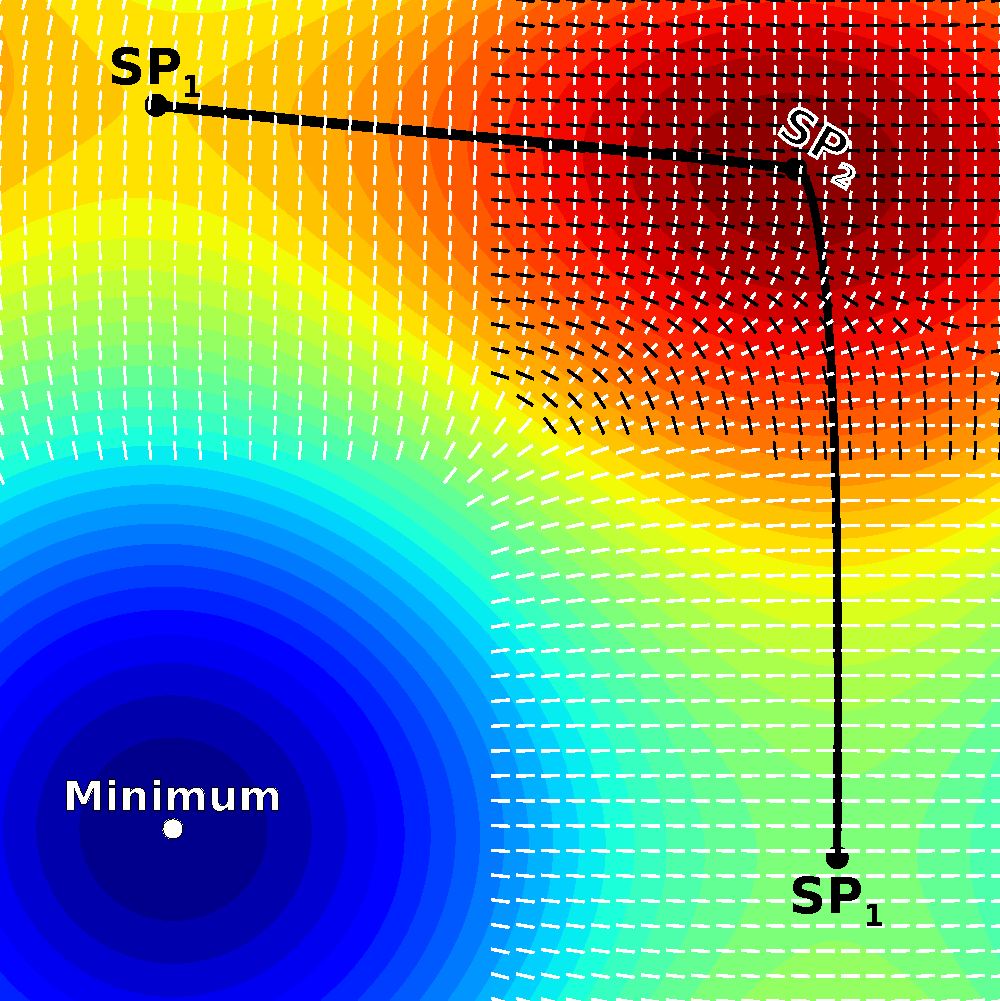
\includegraphics[width=0.5\linewidth]{figures/modes}
\caption{A schematic two-dimensional energy surface illustrating an energy ridge connecting two first order saddle points and lying through a second order saddle point.
The ridge is shown with a black line and was found by carrying out steepest descent paths to find the dividing surface between starting points that lead to different minima (only one of the minima is shown).
The two first order saddle points are marked with \sap{1} and the second order saddle point with \sap{2}.
The direction of eigenmodes corresponding to negative eigenvalues of the Hessian matrix are shown with short line segments, white indicating the one corresponding to the lower eigenvalue and the black corresponding to the higher one.
}
\label{fig:modes}
\end{center}
\end{figure}

The reduced Hessian matrix for the subspace excluding the tangent vector has at each point on the ridge one and only one negative eigenvalue and the corresponding eigenmode $\uvn$, is necessarily orthogonal to the ridge.
The ridge can be located by maximizing the energy along this direction while minimizing in all other directions perpendicular to the ridge.
By transforming the force, $\vF^\perp$, in such a way that it locally, near the ridge, corresponds to that of a MEP
\begin{equation}
\vF^t = \vF^\perp - 2 (\vF^\perp \cdot \uvn) \uvn,
\label{eq:force-mapping}
\end{equation}
an iterative displacement of the path in the direction of $\vF^t$, i.e. a minimization, can be used to locate the ridge.
This mapping of the force makes it possible to employ a method that is similar to a NEB search for a MEP, but by using the transformed force, $\vF^t$, the path converges on a ridge instead.

A numerical implementation of the path optimization requires the introduction of discretisation.
The path is represented by a discrete set of configurations, a set of images of the system,
with coordinates $[\vR_{0}, \vR_{1}, \dotsc, \vR_{N-1}, \vR_{N}]$.
The energy of each image, $i$, is  $E_i \equiv E(\vR_i)$.
Since a discrete representation of the path is used, the path's tangent needs to be approximated at each image.
In NEB calculations, it has been found to be important, for numerical convergence, to use the vector displacement to the higher energy neighbouring image so as to minimize the formation of kinks in the path\cite{neb-tangent-2000}.
This same tangent estimate was also used in the calculations presented here.

In order to perform the force transformation described in \fref{eq:force-mapping}, it is necessary to be able to find the eigenmode associated with the lowest eigenvalue (hereafter referred to as the minimum mode) of the reduced Hessian matrix.
For this purpose we use the dimer method\cite{dimer-original-1999, dimer-olsen-2004} since it gives the minimum mode using only the force as input.  It is also possible to use the Lanczos method for this purpose \cite{dimer-olsen-2004} at a similar computational effort.
For clarity, we rewrite \fref{eq:force-mapping} for each image, $i$
\begin{equation}
\vF_i^t = \vF^\perp_i - 2 (\vF^\perp_i \cdot \uvn_i) \uvn_i,
\label{eq:minmode-force}
\end{equation}
which is applied after the dimer has been rotated subject to a constraint $\uvn_i \cdot \uvt_i =0$ to find the minimum mode of the reduced Hessian matrix.

\begin{figure}[t]
\begin{center}
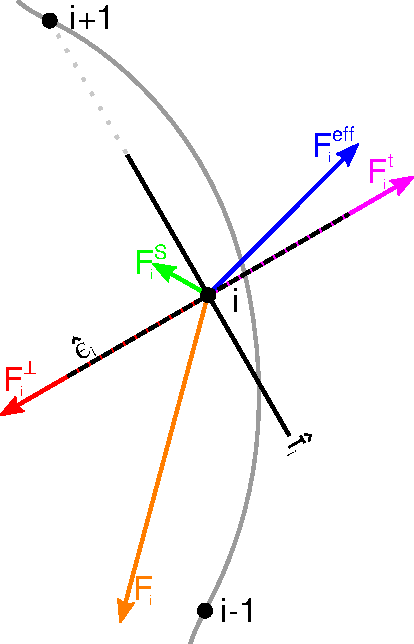
\includegraphics[width=0.5\linewidth]{figures/erm-forces}
\caption{
The construction of the effective force, $\vF_i^\text{eff}$, used in the iterative optimization for finding an energy ridge, from \fref{eq:effective-force}.
$\vF_i$ (orange) is the real force, $\vF_i = -\nabla E_i$ acting on the image,
$\vF^t_i$ (red) is the transformed force, inverted in the direction of the minimum mode, from \fref{eq:minmode-force},
$\vF^\perp_i$ (purple) is the component of the transformed force, $\vF^t_i$, that remains after the component parallel to the tangent has been removed,
$\vF^\text{S}_i$ (green) is the spring force, from \fref{eq:full-spring-force},
$\vF^\text{eff}_i$ (blue) is the effective force acting on the image, from \fref{eq:effective-force}.
For legibility, the image number subscript, $i$, is omitted from all the force symbols.
The solid grey line is the ridge%, the dotted grey line is the current estimate of the ridge
and the black dots represent the current location of the images.}
\label{fig:force-comparison}
\end{center}
\end{figure}

In order to ensure an even distribution of the images along the path, a spring force, $\vF_i^\text{S}$, between adjacent images is introduced.
The force the springs exert on image $i$ is
\begin{equation}
\vF_i^\text{S} = k \left[ \left( \vR_{i+1} - \vR_{i} \right) - \left( \vR_{i} - \vR_{i-1} \right) \right],
\label{eq:full-spring-force}
\end{equation}
where $k$ is the spring constant which can be chosen to fit the energy landscape.
For numerical convergence, it is best to choose $k$ in such a way that the spring force are of roughly the same magnitude as the force derived from the energy surface, but a wide range of values can be used.
Here, the same value of $k$ is used for all pairs of adjacent images, but unequal values can be chosen if an unequal distribution of the images along the ridge is desired, analogous to NEB calculations \cite{neb-ci-2000}.

The effective force, $\vF_i^\text{eff}$, acting on each image can now be written as
\begin{equation}
\vF_i^\text{eff} = \vF_i^t + \vF_i^\text{S}
\label{eq:effective-force}
\end{equation}
where the first term is the transformed force from \fref{eq:minmode-force} and the second term is the spring force from \fref{eq:full-spring-force} that controls the distribution of the images along the path and increases numerical stability.
The construction of the effective force is illustrated in \fref{fig:force-comparison}.

The spring force tends to shorten the path by allowing the component perpendicular to the path to pull it off the ridge.
The position of the images converges to an equilibrium between the components of the spring force and the transformed force that are perpendicular to the tangent,
\begin{equation}
\vF^t_i - (\vF^t_i \cdot \uvt_i)\uvt_i = - (\vF^\text{S}_i - (\vF^\text{S}_i \cdot \uvt_i)\uvt_i)
\end{equation}
If the ridge is curved, this equilibrium will not be exactly at the ridge.
This is referred to as corner-cutting (see, for example \cite{neb-original-1998}).
The perpendicular component of the spring force can be projected out, as is often done in the NEB method, but here it is retained in order to improve the stability of the iterative optimization.

The climbing image algorithm \cite{neb-ci-2000} can be used on the highest energy image of the path to ensure exact convergence to the highest energy \sap{2} along the ridge.
This is accomplished by decoupling the highest energy image from the springs and inverting the force along the tangent in a manner similar to \fref{eq:minmode-force},
\begin{equation}
\vF_{i_\text{max}}^\text{eff} = \vF_{i_\text{max}}^\ddagger - 2 (\vF_{i_\text{max}}^\ddagger \cdot \uvt_{i_\text{max}})\uvt_{i_\text{max}},
\label{eq:neb-ci}
\end{equation}
where $i_\text{max}$ refers to the image with the highest energy.
This decoupling achieves two things.
It allows the highest energy image to converge onto the \sap{2} exactly without significant increase in computational power and it allows the highest energy image to be decoupled from the spring force which, in turn, will allow it to overcome any tendency for corner-cutting.

\begin{figure}[b]
\begin{center}
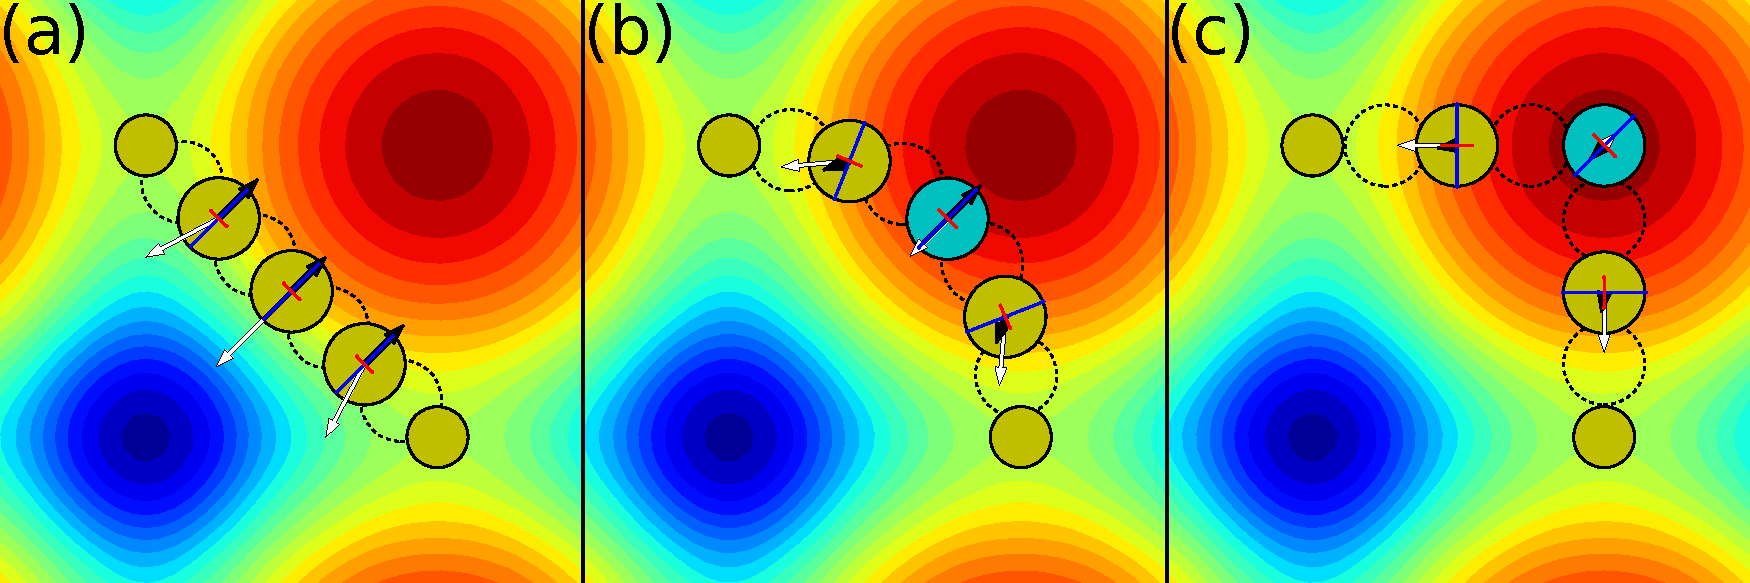
\includegraphics[width=0.8\linewidth]{figures/snapshots}
\caption{Snapshots from an optimization of a path connecting two neighbouring adatom hop \sap{1}s on a 2x2x1 Al(100) slab.
See the supplementary materials for the full animation.
For simplicity, the Al atoms in the slab are kept fixed in this illustrative test problem.
The energy surface is generated by minimizing the energy of the adatom along the normal to the surface plane but keeping the in-plane coordinates fixed.
Each sphere represents a different image in the path. The cyan sphere is the climbing image and the dotted spheres are omitted for clarity.
The arrows represent the in-plane force acting on each image.
White: The force derived from the energy surface, $-\nabla E$.
Black: The effective force, given by \fref{eq:effective-force} or \fref{eq:neb-ci}, which is used in the iterative optimization.
The red lines represent the tangent and the blue lines represent the minimum mode estimate.
The red areas of the surface represent high potential energy and the blue areas low potential energy.
The immobile substrate atoms are located at the centre of the high potential areas.
(a) initial, straight line interpolation between the \sap{1}s, (b) after 19 optimization steps, converged to $0.05\unit{eV/\mAA}$, without climbing image, (c) after 108 steps, converged to $0.001\unit{eV/\mAA}$ with the climbing image algorithm.}
\label{fig:adatom-snapshots}
\end{center}
\end{figure}

A major difference between MEP and ridge calculations is that there is no guarantee that the initial energy profile represents a barrier.
In fact, the initial energy profile of a ridge calculation can be monotonic or even an inverted barrier, e.g. when the initial path lies close to a minimum.
Such ill-behaved profiles can pose stability problems.
and in order to minimize them, the full spring force is used.
Furthermore, complications can arise when turning on the climbing image algorithm as either of the immobile end points might, in fact, have the highest energy.
In such cases it may prove necessary to set an image that is not the highest energy one as the climbing image
The images closest to the end images are partially constrained by the immobility of the end images,
thus an image even further in, $\vR_2$ or $\vR_{N-2}$, must be set as the climbing image.
Once the path reaches the ridge and a barrier is present the highest energy image can, once again, be used as the climbing image.
In cases where little corner cutting takes place or the \sap{2} is not close to either \sap{1}, in energy and/or space,
this is not needed as the path will climb up the ridge until a barrier emerges by itself.
The lack of an intrinsic barrier makes climbing image ridge calculations risky, at best, to run from the initial interpolation.

The efficiency of the minimum mode algorithm is the controlling factor for the efficiency of the ridge calculation.
Roughly, the computational effort in finding a ridge is about three times that of a NEB calculation of a MEP due to the additional force evaluations needed to rotate the dimer.
The ridge calculation converges, furthermore, slower than a MEP calculation
as the dimer estimate of the minimum mode introduces instabilities beyond those from the NEB.

The method described here has been implemented and tested using the Atomic Simulation Environment (ASE)\footnote{https://wiki.fysik.dtu.dk/ase/}~\cite{ase-2002} using both analytical potential energy functions and density functional theory (DFT) to evaluate the atomic force.

\end{comment}

% ------------------------------------------------------------------
\subsection{Energy Ridge Mapping}
\label{sec:energy-ridge-mapping}

In the context of atomic simulations, the function in question is often the potential energy as a function of all atomic co-ordinates.

\incomplete
